\documentclass[unicode]{beamer}

\usepackage{array} % for m column type
\usepackage{amsmath} % align
\usepackage{bbm}
\usepackage{booktabs}
\usepackage{csvsimple} % for \csvreader
\usepackage[utf8]{inputenc}
\usepackage[orientation=portrait,size=a0,scale=1.4]{beamerposter}
\usepackage{graphicx}

\usepackage[style=numeric, sorting=none, url=false, doi=false]{biblatex}
\addbibresource{src/ref.bib}
\AtBeginBibliography{
  \scriptsize
	\setlength{\labelsep}{0pt}
	\renewcommand{\arraystretch}{0.2}
}

\usepackage{tikz}
\usetikzlibrary{
  arrows.meta, % for changing arrow head size
  calc,
  positioning,
  shapes.callouts,
  tikzmark,
}

\newcommand{\ispace}{\mathbb{D}^{m}}
\newcommand{\Prec}{\operatorname{acc}}
\newcommand{\Cov}{\operatorname{cov}}
\newcommand{\cands}{\bar{\mathcal{A}}}
% \algnewcommand{\IIf}[1]{\State\algorithmicif\ #1\ \algorithmicthen\ }
% \renewcommand{\algorithmicrequire}{\textbf{Input:}}
% \renewcommand{\algorithmicensure}{\textbf{Output:}}


\newcommand{\dtrain}{D_{\mathrm{train}}}
\newcommand{\dtest}{D_{\mathrm{test}}}
\newcommand{\dmis}{D_{\mathrm{mis}}}
\newcommand{\dchange}{D_{\mathrm{change}}}

\setbeamercolor{hokudai}{bg=hokudai!20}

\usetheme[footertext={
  27th International Conference on Pattern Recognition, December 01--05, 2024,
  Kolkata, India
  }]{SimplePoster}

\title{
  R-LIME:Rectangular Constraints and Optimization for \\
  Local Interpretable Model-agnostic Explanation Methods
}
\author{Genji Ohara, Keigo Kimura, Mineichi Kudo}
\institute{
  Division of Computer Science and Information Technology \\
  Graduate School of Information Sci\@. and Tech., Hokkaido University
}
\date{\today}

\begin{document}

\begin{frame}
  \vspace{-0.2em}
  \begin{columns}[t]
    \def\lcol{0.375}
    \def\rcol{0.62}
    \hspace{-1.0em}
    \begin{column}{\lcol\linewidth}
      \begin{block}{1. Background}
        \hspace{-0.5em}
        \begin{beamercolorbox}[wd=.52\textwidth,colsep=0.3cm,rounded=true,shadow=true]{hokudai}
          Interpretable Machine Learning
        \end{beamercolorbox}
        \bigskip
        \begin{columns}[]
          \begin{column}{0.4\textwidth}
            {
              \begin{itemize}
                \item simple models
                      \begin{itemize}
                        \item linear models
                        \item decision trees
                      \end{itemize}
              \end{itemize}
            }
            \hspace{0.5em}
            \textrightarrow{} process is \underline{clear}
          \end{column}
          \begin{column}{0.4\textwidth}
            \begin{itemize}
              \item complex models
                    \begin{itemize}
                      \item deep neural networks
                      \item ensemble models
                    \end{itemize}
            \end{itemize}
            \hspace{0.5em}
            \textrightarrow{} process is \underline{unclear}
          \end{column}
        \end{columns}
        \vspace{0.6em}
        \begin{center}
          \underline{Locally approximate complex models by simple models}
        \end{center}
      \end{block}
      \vspace{-0.6em}
      \begin{block}{2. Related Work}
        \hspace{-1.0em}
        \textbf{LIME \small(Local Interpretable Model-agnostic Explanations)}\cite{ribeiro2016why}
        \vspace{-0.6em}
        \begin{columns}
          \begin{column}{.55\textwidth}
            {
              \renewcommand{\leftmargini}{2.5em}
              \begin{enumerate}
                \item Sample perturbed instances around the given focal point
                \item Learn a linear model on the instances
              \end{enumerate}
            }
          \end{column}
          \begin{column}{.45\textwidth}
            \begin{figure}
              \centering
              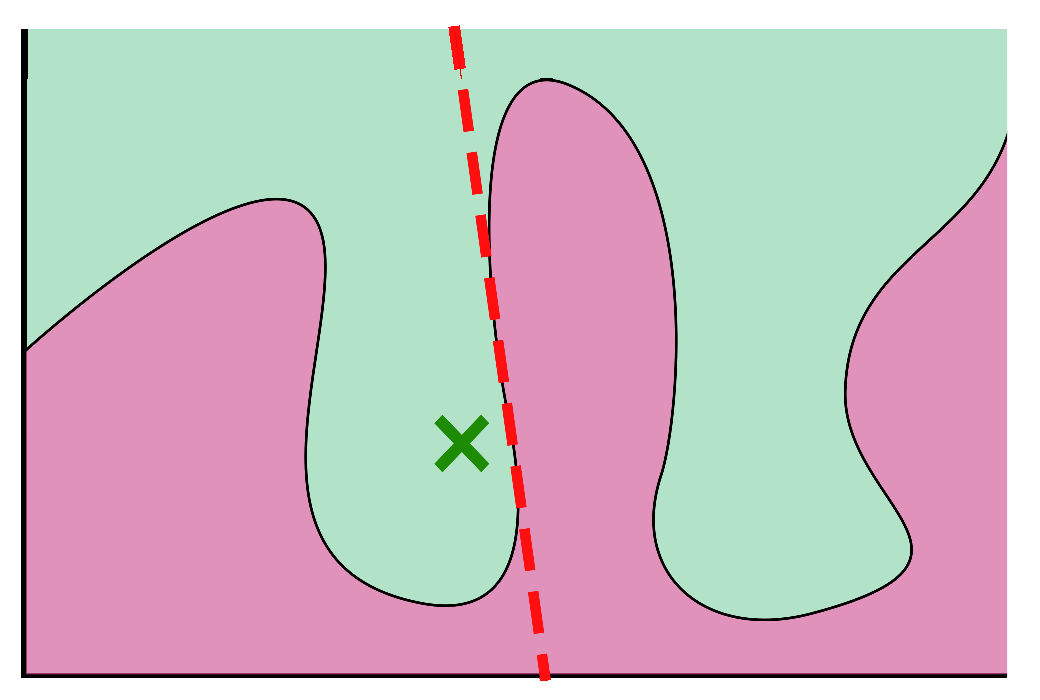
\includegraphics[width=.8\textwidth]{src/img/visual-lime}
            \end{figure}
          \end{column}
        \end{columns}

        \vspace{1.0em}
        \hspace{-1.0em}
        \textbf{Anchor}\cite{ribeiro2018anchors}
        \vspace{-0.5em}
        \begin{columns}
          \begin{column}{.55\textwidth}
            {
              \renewcommand{\leftmargini}{2.5em}
              \begin{enumerate}
                \item Maximize the rectangular region as long as
                      the model’s outputs are consistent with high probability
              \end{enumerate}
            }
          \end{column}
          \begin{column}{.45\textwidth}
            \begin{figure}
              \centering
              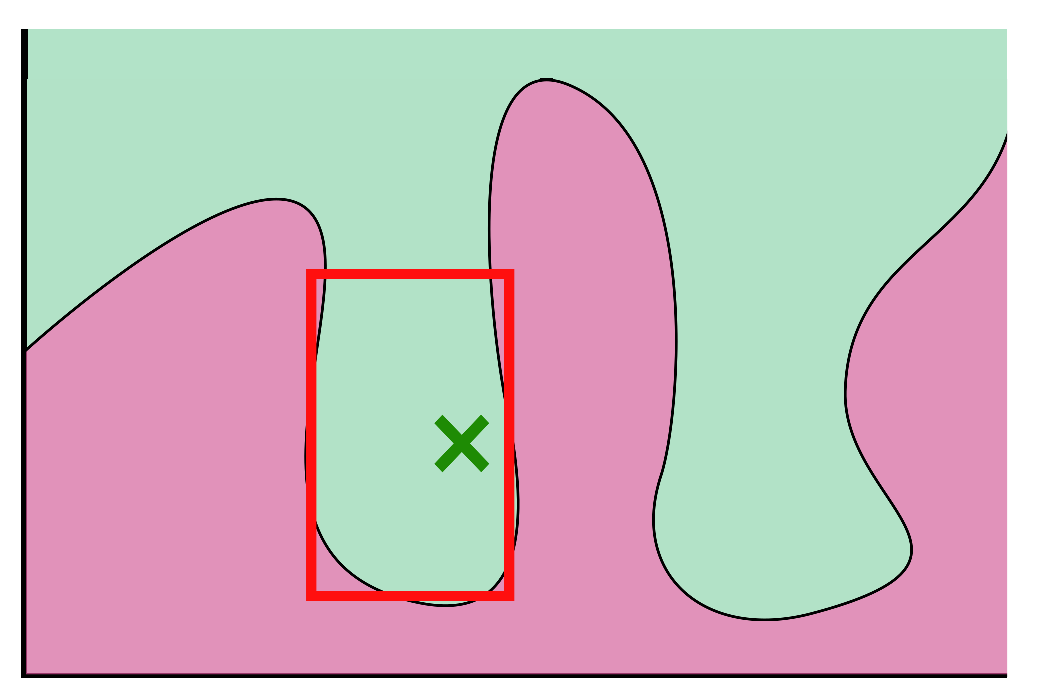
\includegraphics[width=.8\textwidth]{src/img/visual-anchor}
            \end{figure}
          \end{column}
        \end{columns}
        \vspace{1.0em}
        \hspace{-1.0em}
        \textbf{LIME vs. Anchor}
        \vspace{0.5em}
        \begin{columns}[]
          \begin{column}{0.4\textwidth}
            \begin{figure}
              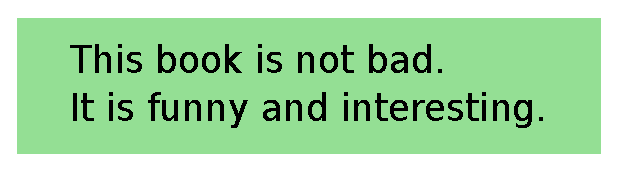
\includegraphics[width=\textwidth]{src/img/example-instance}
              \caption{The focal point}
            \end{figure}
            \vspace{0.5em}
            \begin{figure}
              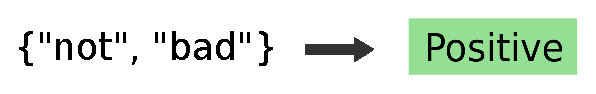
\includegraphics[width=\textwidth]{src/img/example-anchor}
              \caption{Anchor's explanation}
            \end{figure}
          \end{column}
          \begin{column}{0.35\textwidth}
            \begin{figure}
              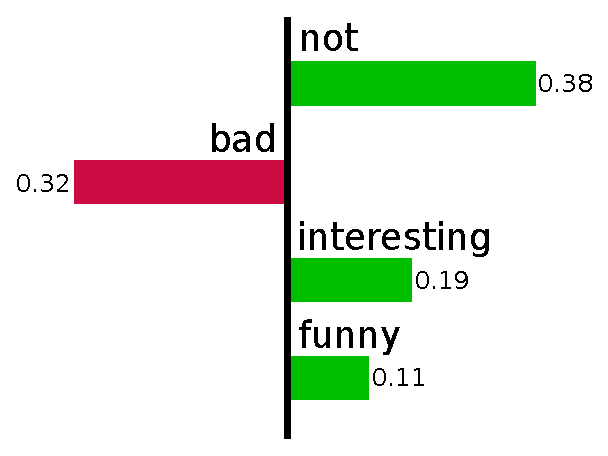
\includegraphics[width=\textwidth]{src/img/example-lime}
              \caption{LIME's explanation}
            \end{figure}
          \end{column}
        \end{columns}
        \vspace{0.3em}
        {
          \begin{center}~%
            \begin{beamercolorbox}[wd=0.7\textwidth,colsep=0.3cm,rounded=true,shadow=true]{hokudai}
              \vspace{-0.2em}
              \begin{itemize}
                \item LIME\@: unclear and not optimal scope
                \item Anchor: users get less insight
              \end{itemize}
              \vspace{0.1em}
            \end{beamercolorbox}~%
          \end{center}
        }
        \vspace{-0.25em}
      \end{block}
    \end{column}
    \begin{column}{\rcol\textwidth}
      \begin{block}{3. Proposed Method}
        \begin{columns}[]
          \begin{column}{0.6\textwidth}
            \begin{beamercolorbox}[wd=.77\textwidth,colsep=0.3cm,rounded=true,shadow=true]{hokudai}
              \textbf{R-LIME (Ruled LIME)} = LIME + Anchor
            \end{beamercolorbox}
            \vspace{0.3em}
            \begin{itemize}
              \item Approximate in rectangular region
              \item Maximize the region as long as approximation accuracy is
                    higher than the given threshold
              \item Express the region as a conjunction of feature predicates \\[0.5em]
                    \hspace{0.2em}\small{
                      ex. $\textrm{Gender} = \textrm{'Male' AND } 20\le\textrm{Age} < 30$
                    }
            \end{itemize}
          \end{column}
          \begin{column}{0.3\textwidth}
            \begin{figure}
              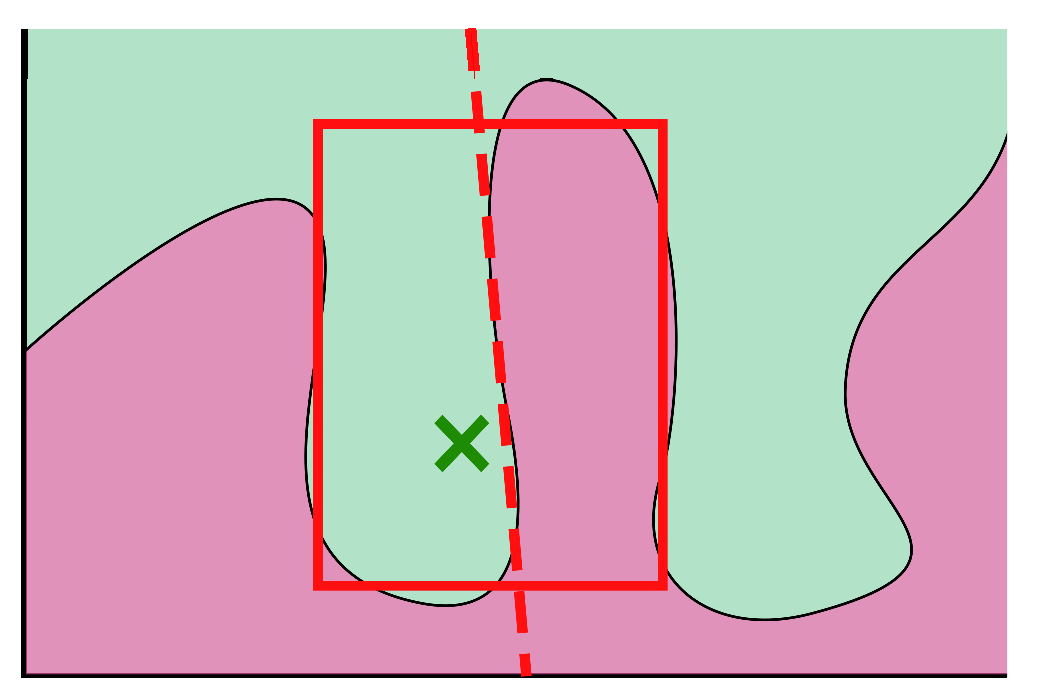
\includegraphics[width=\textwidth]{src/img/visual-rlime3}
            \end{figure}
          \end{column}
        \end{columns}

        \vspace{1.0em}
        \begin{columns}[t]
          \def\lcol{0.50}
          \def\rcol{0.48}
          \begin{column}{\lcol\textwidth}
            \underline{\textbf{Settings}}
            \begin{align*}
               & \text{input space (discretized)}   &  & \ispace             \\
               & \text{a black-box classifier}      &  & f:\ispace\to\{0,1\} \\
               & \text{a focal point}               &  & x\in\ispace         \\
               & \text{distribution on input space} &  & \mathcal{D}         \\
               & \text{all possible approx.\ model} &  & G
            \end{align*}

            \vspace{0.8em}
            \underline{\textbf{Definitions}}

            \vspace{1.0em}
            \begin{columns}
              \begin{column}{0.95\textwidth}
                rule: a conjunction of predicates
                \begin{align*}
                  A(z)   & =a_{i_1}(z)\wedge a_{i_2}(z)\wedge\dots\wedge a_{i_k}(z) \\
                  a_i(z) & =\mathbbm{1}_{z_i=x_i}
                \end{align*}
                accuracy: expected accuracy of approx.\ $g$ in $A$
                \begin{equation*}
                  \Prec(A)=\underset{g\in G}{\max}
                  \ \mathbb{E}_{z\sim\mathcal{D}(z|A)}[\mathbbm{1}_{f(z)=g(z)}]
                \end{equation*}
                coverage: probability that sample $z$ is inside $A$
                \begin{equation*}
                  \operatorname{cov}(A)=
                  \mathbb{E}_{z\sim\mathcal{D}(z)}[A(z)]
                \end{equation*}
                our problem:

                \vspace{0.2em}
                \begin{center}~%
                  \begin{beamercolorbox}[wd=.85\textwidth,colsep=0.1cm,rounded=true,shadow=true]{hokudai}
                    \begin{center}
                      $
                        \tilde{A}=\underset{A\ s.t.
                          \ P(\Prec(A)\ge\tau)\ge1-\delta,A(x)=1}  % chktex 36
                        {\arg\max}\operatorname{cov}(A)  % chktex 36
                      $
                    \end{center}~%
                  \end{beamercolorbox}

                  \vspace{0.5em}
                  \underline{Maximize coverage under constraint of accuracy}
                \end{center}
                \vspace{0.8em}
                \begin{figure}[t]
                  \centering
                  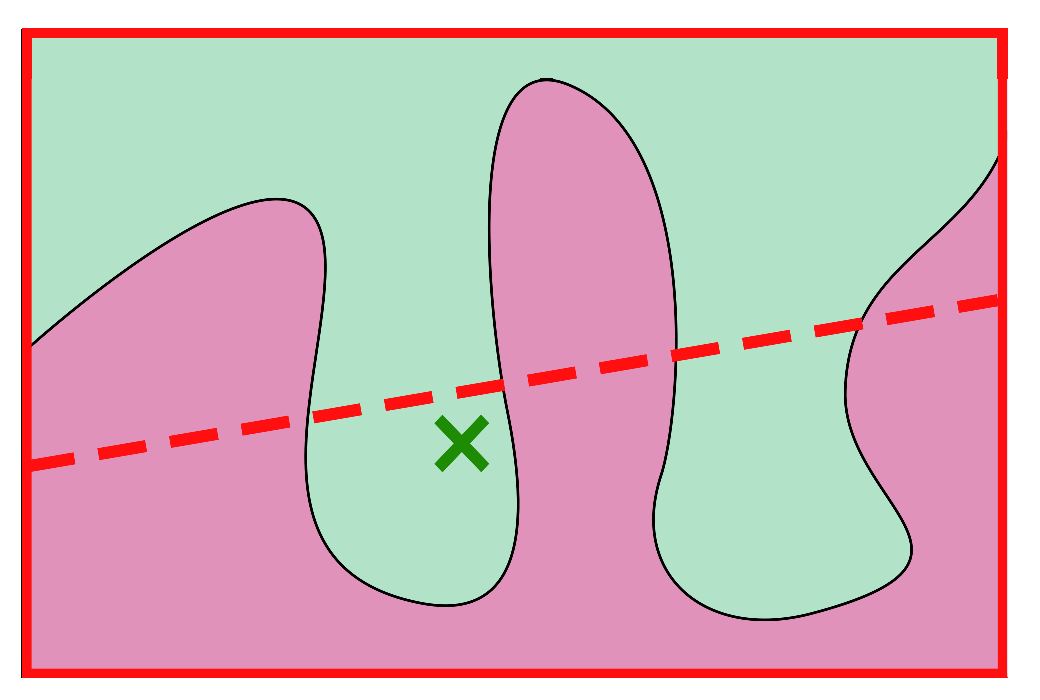
\includegraphics[width=0.3\textwidth]{src/img/visual-rlime1}
                  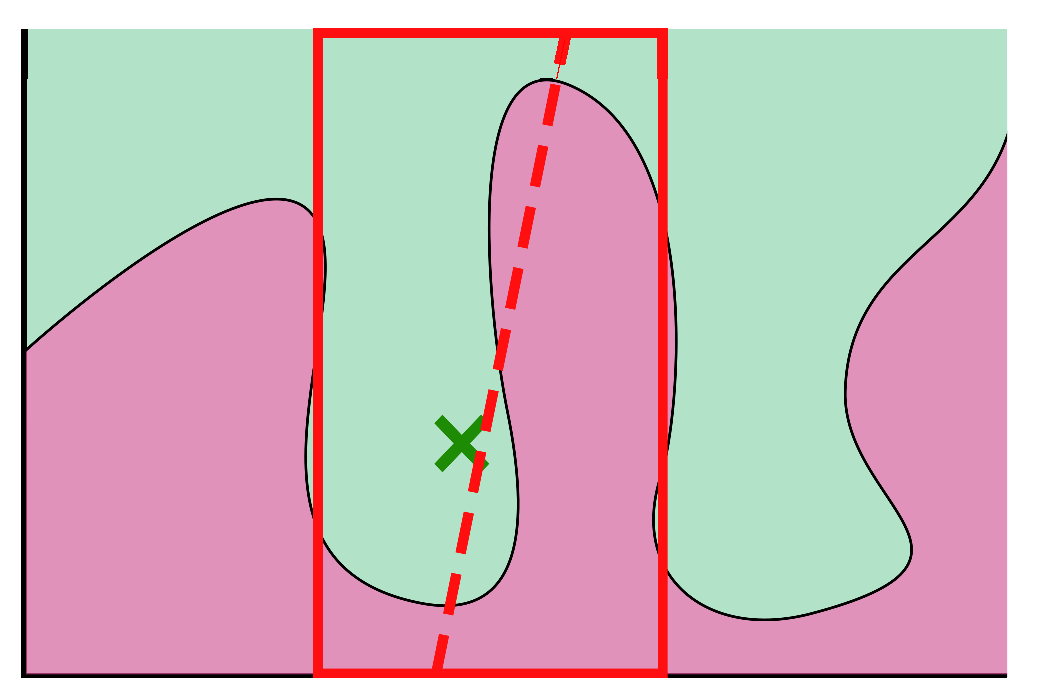
\includegraphics[width=0.3\textwidth]{src/img/visual-rlime2}
                  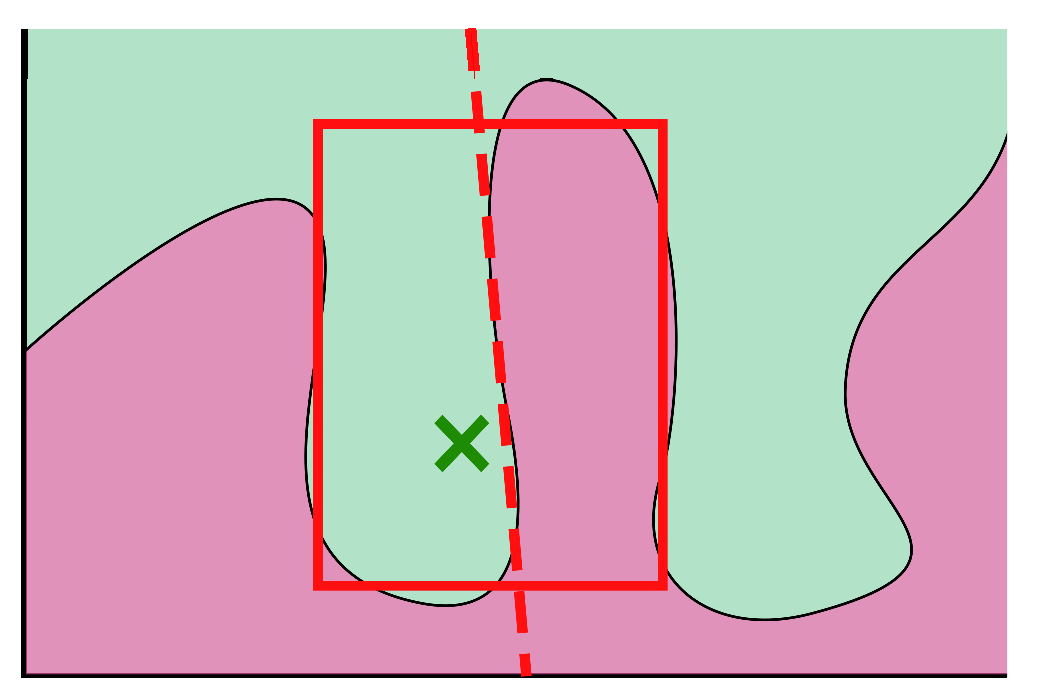
\includegraphics[width=0.3\textwidth]{src/img/visual-rlime3}
                \end{figure}
              \end{column}
            \end{columns}
          \end{column}
          \begin{column}{\rcol\textwidth}
            \hspace{-1.0em}
            \underline{\textbf{Algorithm}} (beam search)

            \vspace{1.0em}
            $\mathcal{A}_{t-1}=\{A_1,\ldots,A_B\}$
            \begin{tikzpicture}
              \node (a) {};
              \node [below = 6cm of a] (b) {};
              \draw [-{Latex[length=5mm, width=5mm]}] (a) to node[right] {
                  \begin{beamercolorbox}[wd=.8\textwidth,colsep=0.2cm,rounded=true,shadow=true]{hokudai}
                    Generate a set of candidate rules
                    \small
                    \begin{itemize}
                      \item add a new predicate to each rule\\
                            $\mathcal{A}_{t-1}=\{a_1\}$\\
                            $\rightarrow\mathcal{A}_t=\{a_1\wedge a_2,
                              a_1\wedge a_3,a_1\wedge a_4,\dots\}$
                    \end{itemize}
                  \end{beamercolorbox}
                } (b);
            \end{tikzpicture}
            $\bar{\mathcal{A}}_{t}=\{A_1\wedge a_1,A_1\wedge a_2,\ldots,A_B\wedge a_m\}$
            \begin{tikzpicture}
              \node (a) {};
              \node [below = 6cm of a] (b) {};
              \draw [-{Latex[length=5mm, width=5mm]}] (a) to node[right] {
                  \begin{beamercolorbox}[wd=.8\textwidth,colsep=0.2cm,rounded=true,shadow=true]{hokudai}
                    Search rules with highest accuracy
                    \small
                    \begin{itemize}
                      \item solve as best arm identification in multi-armed
                            bandit problem using KL-LUCB algorithm\cite{kaufmann2013information}
                    \end{itemize}
                  \end{beamercolorbox}
                } (b);
            \end{tikzpicture}
            $\mathcal{A}_t=\{A'_1,A'_2,\ldots,A'_B\}$
            \begin{tikzpicture}
              \node (a) {};
              \node [below = 6cm of a] (b) {};
              \draw [-{Latex[length=5mm, width=5mm]}] (a) to node[right] {
                  \begin{beamercolorbox}[wd=.8\textwidth,colsep=0.2cm,rounded=true,shadow=true]{hokudai}
                    Search a rule with highest coverage under constraint of accuracy
                    \small
                    \begin{itemize}
                      \item sample and update bounds $\Prec_u,\Prec_l$ unless
                            $\Prec(A)_u\le\tau$ or $\tau\le\Prec(A)_l$
                    \end{itemize}
                  \end{beamercolorbox}
                } (b);
            \end{tikzpicture}
            $A^*=\underset{
                A\in\mathcal{A}_t \ s.t. \ P(\Prec(A)\ge\tau)\ge1-\delta
              }{\arg\max}\operatorname{cov}(A)$
            \begin{tikzpicture}
              \node (a) {};
              \node [below = 6.0cm of a] (b) {};
              \node [below = 0.5cm of a] (c) {};
              \node [right = 13.0cm of c, align=left] (d) {$t\gets t+1$;\\continue;};
              \draw [-{Latex[length=5mm, width=5mm]}] (a) to node[below right] {
                  if $A*$ is not null
                } (b);
              \draw [-{Latex[length=5mm, width=5mm]}] (c) to node[below] {
                  if $A*$ is null
                } (d);
            \end{tikzpicture}

            \vspace{-0.8em}
            return $A^*$
          \end{column}
        \end{columns}
      \end{block}
    \end{column}
  \end{columns}
  \begin{columns}[t]
    \def\lcol{0.69}
    \def\rcol{0.30}
    \hspace{-1.0em}
    \begin{column}{\lcol\textwidth}
      \begin{block}{4. Experiments}
        \def\index{0012}
        \vspace{-0.4em}
        \begin{columns}[t]
          \begin{column}{.31\textwidth}
            \vspace{1.0em}
            \begin{figure}[tbp]
              \centering
              {
                \tiny
                \fontfamily{cmtt}\selectfont
                \begin{tabular}{p{10em}m{14em}}
                  \toprule
                  \csvreader[no head, late after line= \\]{%
                    src/experiments/exp1/\index.csv
                  }{}{%
                  \ifnum\thecsvrow=16 \midrule\fi\csvcoli & \csvcolii % chktex 1
                  }
                  \bottomrule
                \end{tabular}
              }
              \vspace{1.0em}
              \caption{Focal point}
            \end{figure}
          \end{column}
          \begin{column}{.290\textwidth}
            \vspace{0.5em}
            \begin{figure}
              \includegraphics[width=\textwidth]{src/experiments/exp1/lime-\index}
              \caption{LIME's explanation}
            \end{figure}
            \vspace{0.2em}
            \begin{figure}
              \includegraphics[width=\textwidth]{src/experiments/exp1/anchor-\index-70}
              \vspace{-1.8em}
              \caption{Anchor's explanation ($\tau=0.70$)}
            \end{figure}
          \end{column}
          \begin{column}{.295\textwidth}
            \vspace{-0.4em}
            \begin{figure}
              \includegraphics[width=\textwidth]{src/experiments/exp1/rlime-\index-70}

              \vspace{-0.1em}
              \caption{R-LIME's explanation ($\tau=0.70$)}
            \end{figure}
            \vspace{0.8em}
            \begin{beamercolorbox}[colsep=0.1cm,rounded=true,shadow=true]{hokudai}
              \begin{itemize}
                \setlength{\itemsep}{0.3em}
                \item More interpretable and optimal than LIME
                \item More descriptive than Anchor
              \end{itemize}
              \vspace{0.5em}
            \end{beamercolorbox}
          \end{column}
        \end{columns}
        \begin{columns}
          \def\lcol{0.620}
          \def\rcol{0.295}
          \begin{column}{\lcol\textwidth}
            \vspace{-2.5em}
            \begin{columns}[t]
              \begin{column}{.509\textwidth}
                \begin{figure}
                  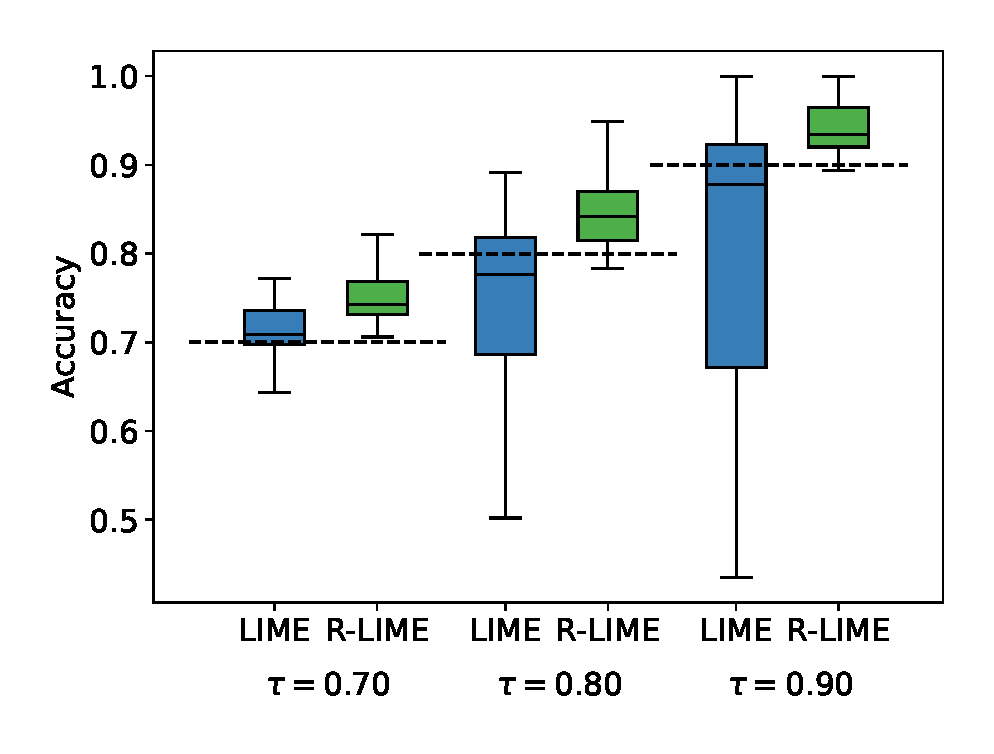
\includegraphics[width=.88\textwidth]{src/experiments/exp2/box_plot}
                  \vspace{-0.4em}
                  \caption{LIME vs. R-LIME (in accuracy)}
                \end{figure}
              \end{column}
              \begin{column}{.491\textwidth}
                \begin{figure}
                  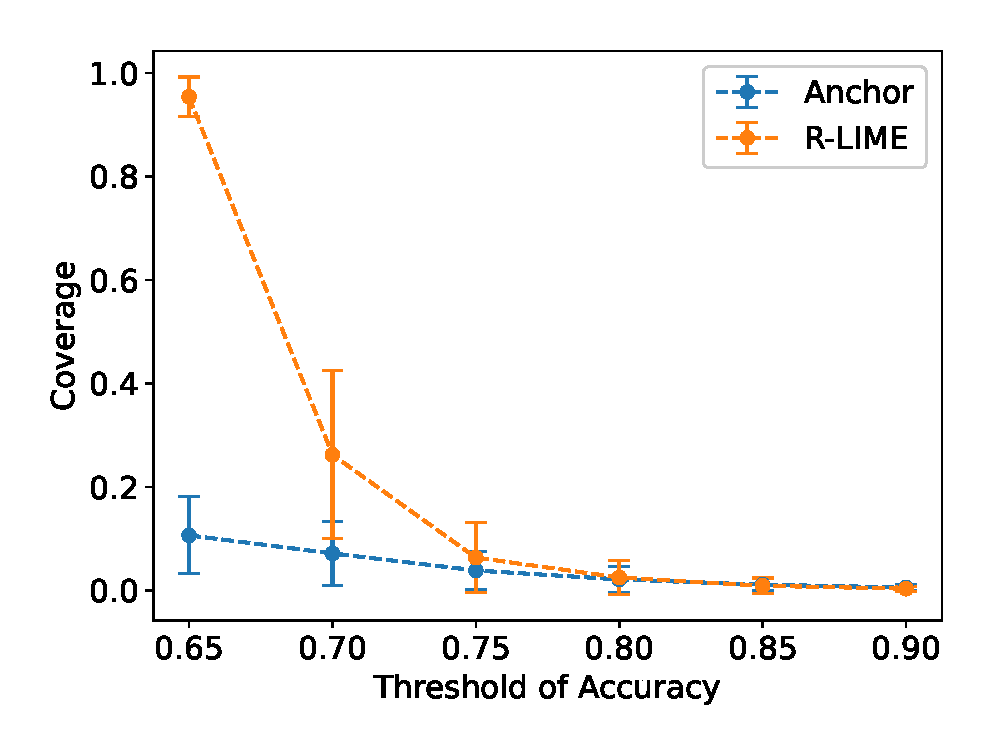
\includegraphics[width=.88\textwidth]{src/experiments/exp2/comp_cov}
                  \caption{LIME vs. R-LIME (in coverage)}
                \end{figure}
              \end{column}
            \end{columns}
          \end{column}
          \begin{column}{\rcol\textwidth}
            \vspace{0.5em}
            \begin{beamercolorbox}[colsep=0.1cm,rounded=true,shadow=true]{hokudai}
              \begin{itemize}
                \setlength{\itemsep}{0.3em}
                \setlength{\parskip}{0.2em}
                \item More accurate than LIME
                      \begin{itemize}
                        \item R-LIME adapts to optimized region flexibly
                      \end{itemize}
                \item More general than Anchor
                      \begin{itemize}
                        \item R-LIME captures decision boundary more plecisely
                      \end{itemize}
              \end{itemize}
            \end{beamercolorbox}
          \end{column}
        \end{columns}
      \end{block}
    \end{column}
    \begin{column}{\rcol\textwidth}
      \begin{block}{5. Conclusion}
        \renewcommand{\arraystretch}{1.4}
        \tabcolsep=0.6em
        \begin{center}
          \small
          \begin{tabular}{cccc}
                                & LIME         & Anchor       & \textbf{R-LIME} \\
            \midrule
            Feature Importance  & \checkmark{} & $\times$     & \checkmark{}    \\
            Optimal Scope       & $\times$     & \checkmark{} & \checkmark{}    \\
            Interpretable Scope & $\times$     & \checkmark{} & \checkmark{}    \\
          \end{tabular}
        \end{center}

        % NOTE: center environment does not work here.
        %       we use columns environment instead.
        %       cf. https://tex.stackexchange.com/a/7441
        \vspace{0.5em}
        \begin{columns}
          \begin{column}{0.8\textwidth}
            \begin{beamercolorbox}[wd=\textwidth,colsep=0.3cm,rounded=true,shadow=true]{hokudai}
              \vspace{-0.3em}
              \begin{itemize}
                \item Achieved interpretability of both explanation and its scope! \\ [0.8em]
                      Also:
                      \begin{itemize}
                        \item More accurate than LIME
                        \item More general than Anchor
                      \end{itemize}
              \end{itemize}
            \end{beamercolorbox}~%
          \end{column}
        \end{columns}
      \end{block}
      \vspace{-0.6em}
      \begin{block}{References}
        \vspace{-0.6em}
        \begin{columns}[t]
          \begin{column}{0.99\textwidth}
            \printbibliography{}
          \end{column}
          \begin{column}{0.01\textwidth}
          \end{column}
        \end{columns}
        \vspace{-0.4em}
      \end{block}
    \end{column}
  \end{columns}
\end{frame}

\end{document}
